%!TEX root = thesis.tex

\documentclass[a4paper]{article}
\usepackage{amsthm}
\usepackage[utf8]{inputenc}
\usepackage{csquotes}
\usepackage[english]{babel}
\usepackage{graphicx}
\usepackage{enumitem}
\usepackage{subcaption}  %ALLOWS SUBFIGURES
\usepackage{wrapfig}

\usepackage[draft]{fixme}
\fxsetup{theme = color}
\definecolor{fxnote}{rgb}{0.0000, 0.6000,0.0000}
\definecolor{fxwarning}{rgb}{1.0000,0.5490,0.0000}
\definecolor{fxerror}{rgb}{1.0000,0.2706,0.0000}
\definecolor{fxfatal}{rgb}{1.0000,0.0000,0.0000}
\usepackage[backend=biber, giveninits =true, isbn=false, url=false, maxbibnames=100]{biblatex}
\usepackage{hyperref}

%Theorems
\newtheorem{thrm}{Theorem}
\newtheorem{lemma}[thrm]{Lemma}
\newtheorem{prop}[thrm]{Proposition}
\newtheorem{remark}[thrm]{Remark}

\theoremstyle{definition}
\newtheorem*{defi}{Definition}

%%BeginIpePreamble
\usepackage{amsmath}
\usepackage{amssymb}
\usepackage{amsopn}

\newcommand{\scr}[1]{\mathcal{#1}}
\newcommand{\Z}{\mathbb{Z}}
\newcommand{\F}{\mathbb{F}}
\newcommand{\R}{\mathbb{R}}
\newcommand{\N}{\mathbb{N}}
\newcommand{\Q}{\mathbb{Q}}


%Operators
\newcommand{\id}{\operatorname{Id}}



%braces etc
\newcommand{\braces}[1]{\left\lbrace {#1} \right\rbrace}
\newcommand{\sqbr}[1]{\left\lbrack {#1} \right\rbrack }
\newcommand{\abs}[1]{\left\lvert {#1} \right\rvert }
\newcommand{\ceil}[1]{\left\lceil{ #1 } \right\rceil}
\newcommand{\floor}[1]{\left \lfloor {#1}\right\rfloor}
\newcommand{\parens}[1]{\left( {#1} \right)}


%utility
\newcommand{\inv}[1]{{#1}^{-1}}
\newcommand{\half}{\frac{1}{2}}
\newcommand{\third}{\frac{1}{3}}
\newcommand{\goes}{\rightarrow}
\newcommand{\nin}{\not \in}
\newcommand{\sm}[1]{\setminus \braces{#1} }

%vectors and matrices
\newcommand{\zerov}{\vec{0}}
\newcommand{\onev}{\vec{1}}

\newcommand{\twovec}[2]{\parens{ \begin{array}{c}#1 \\ #2\end{array} }}
\newcommand{\threevec}[3]{\prens{ \begin{array}{c}#1 \\ #2\\#3 \end{array} }}
\newcommand{\fourvec}[4]{\parens{ \begin{arr\newcommand{\ifftext}{if and only if }ay}{c}#1 \\ #2\\#3\\#4 \end{array} }}
\newcommand{\twomatrix}[4]{\parens{\begin{array}{cc}#1 & #2 \\ #3 & #4 \end{array}  }}
\newcommand{\twodiagmatrix}[2]{\parens{\begin{array}{cc}#1 & 0 \\ 0 & #2 \end{array}  }}

%%%%THIS THESIS
\newcommand{\intplus}{\operatorname{Int^{+}}}
\newcommand{\interior}{\operatorname{Int}}
\newcommand{\spl}{\operatorname{split}}
\newcommand{\mrg}{\operatorname{merge}}


\newcommand{\ext}[1]{\bar{#1}}
\newcommand{\tightext}[1]{\bar{#1}_t}
\newcommand{\dualgraph}[1]{\G(#1)}
\newcommand{\extdualgraph}[1]{\G_{\scr E}(#1)}



\newcommand{\W}{\scr W}
\renewcommand{\P}{\scr P}
\newcommand{\C}{\scr C}
\newcommand\restrict[1]{\raisebox{-.5ex}{$|$}_{#1}}
\newcommand{\restC}[1]{\ensuremath{\C\restrict{#1}}}

%p is for pole
\newcommand{\pN}{\mathrm{N}}
\newcommand{\pS}{\mathrm{S}}
\newcommand{\pE}{\mathrm{E}}
\newcommand{\pW}{\mathrm{W}}

\newcommand{\cpath}{\C \setminus \braces{\pS}} %cycle path

\newcommand{\rel}{\text{regular edge labeling }}

%%EndIpePreamble


%bib stuff
\bibstyle{plain}



\begin{document}
\maketitle

%Depracted
\newcommand{\mrN}{\mathrm{N}}
\newcommand{\mrS}{\mathrm{S}}
\newcommand{\mrE}{\mathrm{E}}
\newcommand{\mrW}{\mathrm{W}}


\paragraph{Notational concerns}
We will use $\C$ to indicate the current sweep line cycle. 
We will repeatedly only consider the path $\cpath$. In that case we will always order it from $\mrW$ to $\mrE$. 

We will let $\W$ denote a interior walk  \fxnote{have i defined this already}. Given such a walk of $k$ vertices we index it's nodes $w_1, \ldots, w_k$  in such a way that $w_1$ is closer to $W$ then $w_k$ is (and thus that $w_k$ is closer to $E$ then $w_1$ is). 

Then $w_1$ and $w_k$ indicate the two unique vertices of the walk that are also part of the cycle. We will then let $\restC{\W}$ denote the part of $\C\setminus {\mathrm{S}}$ that is between $w_1$ and $w_k$ (including). $\C_\W$ will denote the closed walk formed when we paste $\restC{W}$ and $\W$.

Since paths are a subclass of walks all of the above notation can also be used for a path $\P$. Note that the closed walk $\C_\P$ in this case will actually be a cycle.


\paragraph{prelim}
\emph{nondistinct corner.}

\section{Outline}
We will show that there is a algorithm if there are no $4$ cycles.

If graph $G$ has non-distinct corners or cutvertices we treat them separately.


The main algorithm will recieve as input a extended graph $\ext G$ without non-distinct corners and no separating $4$ cycles and will return a regular edge labeling such that all red faces are $(1-\infty)$ using a sweepcycle approach inspired by \Fusy \fxnote{spelling Fusy and cite} \cite{F}.

We will start by creating a walk $W$. This walk may not be a valid path, it doesn't even have to be a path. During the algorithm we will make a number of moves that will turn this candidate walk into a valid path. In each move we shrink $C$ by employing a valid path and change the candidate walk.

One invariant we will always maintain is that the area bounded by $\C_\W$ will never have interior vertices. \fxnote{What is exactly the area bounded by a closed walk}.

\subsection{The initial candidate walk}
Let $v_i$ denote all the vertices of $\C \setminus \braces{\pW, \pS, \pE}$ in the order that they occur on $\cpath$.  That is $\cpath$ is given by $\mrW v_1 \ldots v_n \mrE$. 
As candidate walk we will start with $\pW$, we will then take the vertices adjacent to $v_1$ between $\pE$ and $v_2$ in clockwise order (exclusive), followed the vertices adjacent to $v_2$ between $v_1$ and $v_3$ in clockwise order and so further until we finally add the vertices adjacent to $v_n$ between $v_{n-1}$ and $\pE$ in clockwise order and finally we finish by adding $E$.

\begin{lemma}
After removing subsequent duplicates the collection $W$ described above is indeed a walk.
\end{lemma}

\fxnote{introduce a term for "edges subsequent to each other in clockwise order around $v$"}

\begin{proof}
To show that $W$ is a walk it's sufficient to show that every vertex is adjacent to the next vertex. Let us suppose that $w$ and $w'$ are two subsequent vertices in $W$, we will show that they are connected if $\braces{w, w'} \cap \braces{\pW, \pE} = \emptyset$ after that we will consider this edge case. There are then two main case for $w, w'$. Either $(a)$ $w$ and $w'$ are  vertices adjecent to some $v_i$ subsequent in clockwise order or $(b)$ $w$ was the last vertex adjecent to some $v_i$ and thus $w'$ is the first vertex adjacent to $v_{i+1}$.

The following two situations can also be seen in Figure \ref{fig:walkproof}.

\begin{figure}
    \centering
    \begin{subfigure}[b]{0.5\linewidth}
        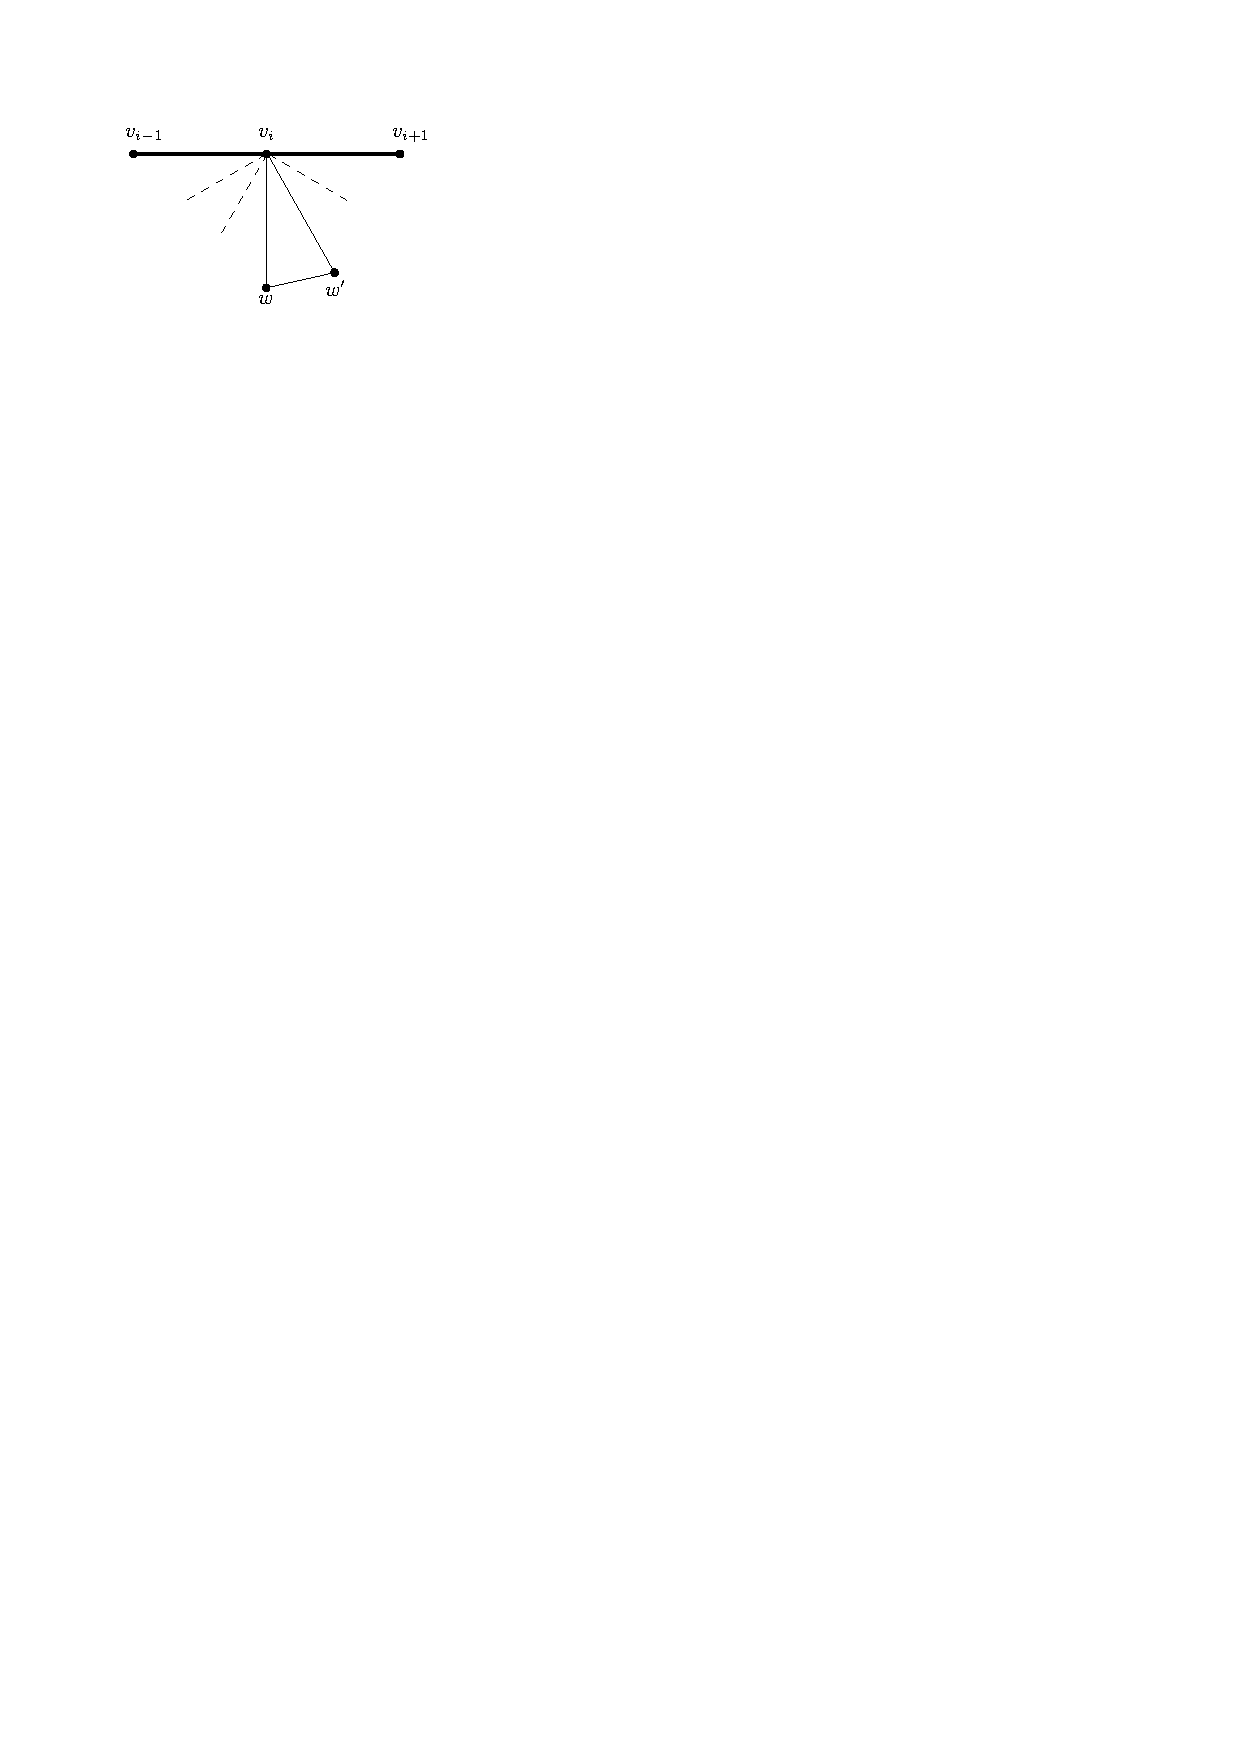
\includegraphics[width=\linewidth]{img/walkProofA}
        \caption{}
    \end{subfigure}%
    \begin{subfigure}[b]{0.5\linewidth}
        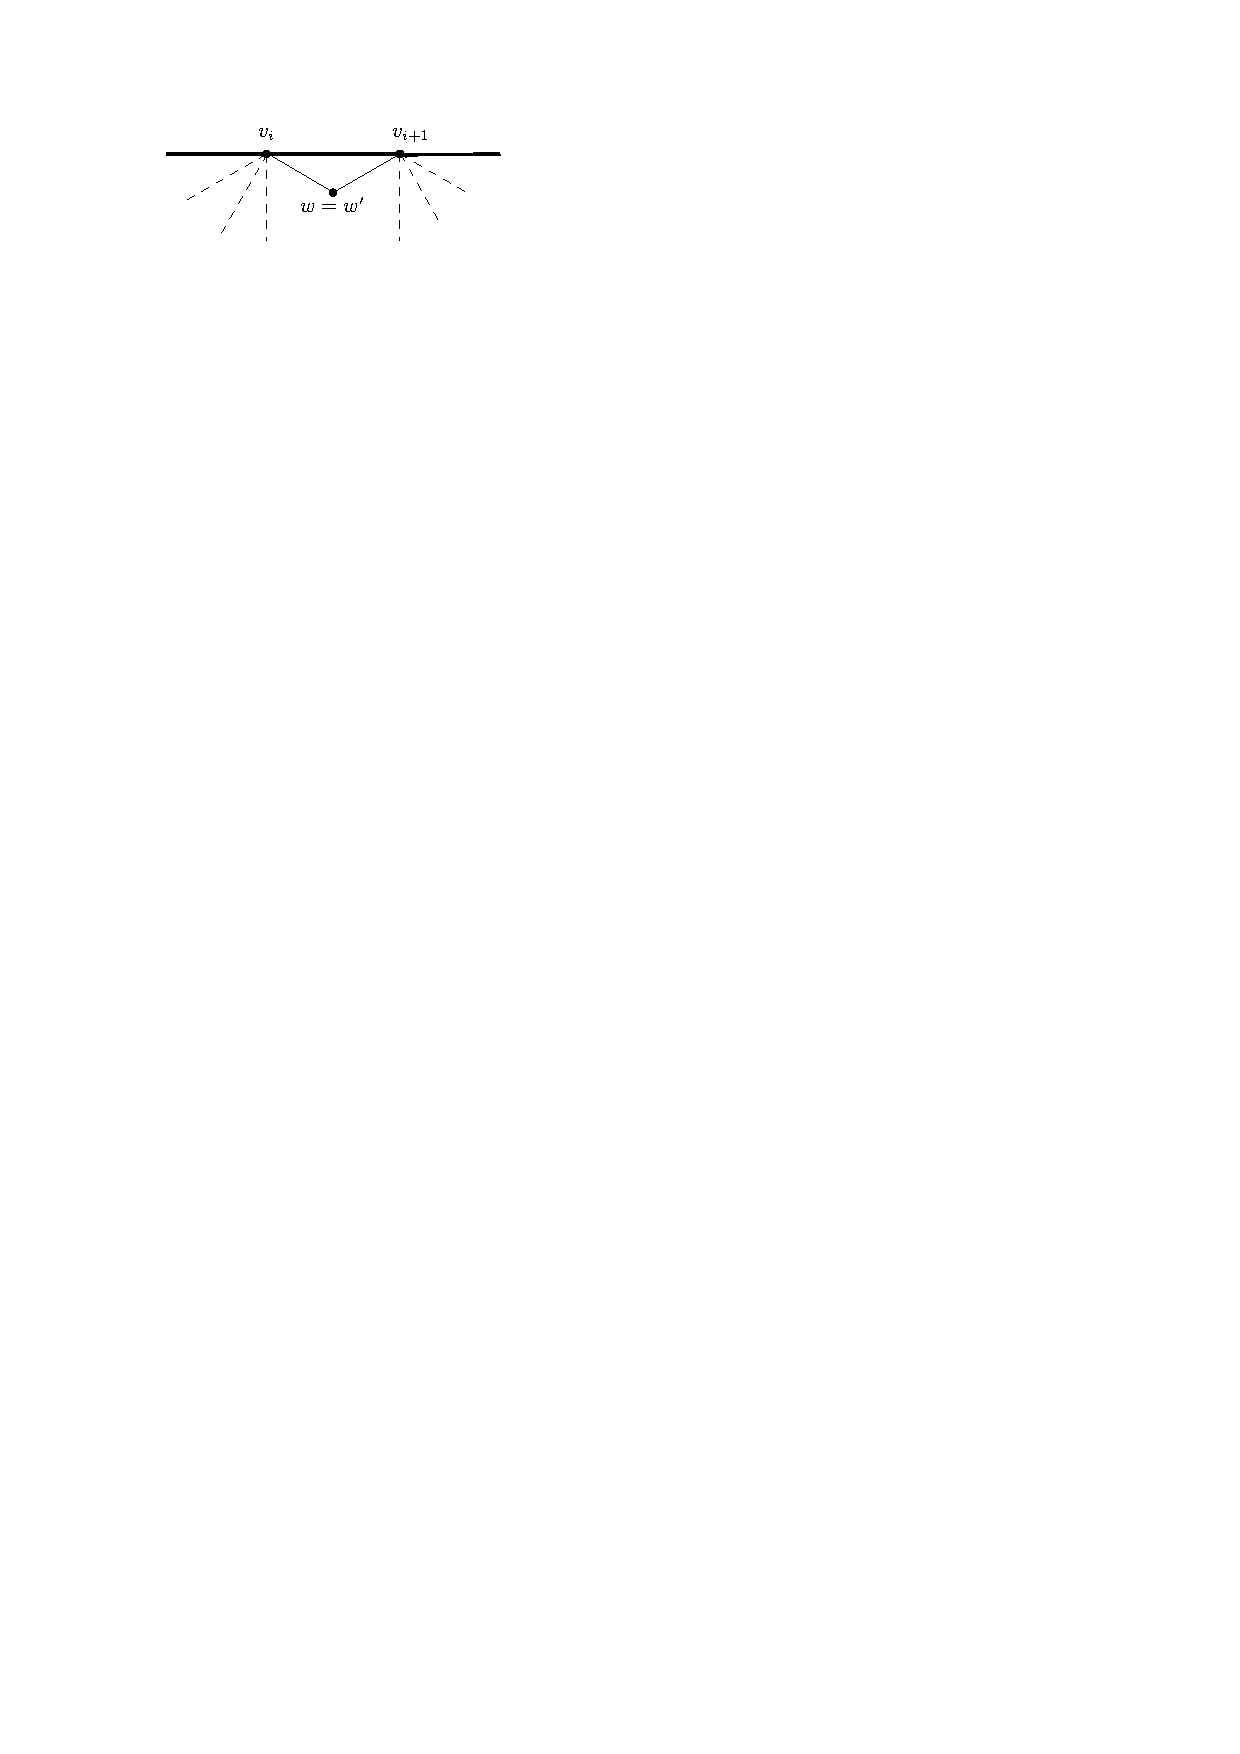
\includegraphics[width=\linewidth]{img/walkProofB}
        \vspace{1cm}   
                
        \caption{}
    \end{subfigure}

    	\caption{The two main cases of the proof showing that $W$ is a walk after removing duplicates.}
	\label{fig:walkproof}
\end{figure}


In case $(a)$ we note that $v_i w$ and $v_i w'$ are edges next to each other in clockwise order around $v_i$. Since every interior face of $\ext G$ is a triangle $ww'$ must be an edge. We thus see that $w, w'$ are adjacent and not duplicates.

In case $(b)$ we note that $v_i w$ and $v_i v_{i+1}$ are edges subsequent in clockwise order, hence $wv_{i+1}$ is also an edge. Hence $w$ is the first vertex adjacent to $v_{i+1}$ after $v_i$ in clockwise order. Thus $w= w'$, they are duplicates and we will remove $w$.

Now for the edge cases: $\pW$ and $w_1$ are vertices adjacent to $v_1$ subsequent in clockwise order, and hence connected. $w_m$ and $\pE$ are vertices adjacent to $v_n$ subsequent in clockwise order and hence connected. 
\end{proof}


\subsection{Porperties the walk already satisfies}

\begin{lemma}
$\C_\W$ has no interior vertices.
\end{lemma}

\begin{lemma}
$\restC\W$ has no chords
\end{lemma}
\begin{proof}
This follows directly from $\C$ having no chords.
\end{proof}

It is clear that both paths have interior vertices

\begin{lemma}
S3 is satisfied since the walk is from $\pW$ to $\pE$
\end{lemma}

\subsection{Moves}

The candidate walk can have two kinds of problems. It either is non-simple or it has chords.\fxnote{cf Kusters. Where there are also two problems for a proper boundary path} Otherwise it is a valid path.



\end{document}